In this section we report the observed and expected upper limits using the entire 
LP dataset corresponding to 1.5~$\ifb$ data. The only difference compared to the 
results repported in Section~\ref{app:lp_limits_default} is the additional cut on the 
transverse mass discussed in Section~\ref{app:lp_technical_changes}. 

Figure~\ref{fig:limits_lp_mtcut80_cut} shows the upper limits for the cut-based analysis, 
with the results tabulated in Table~\ref{tab:limits_lp_mtcut80} 
and Table~\ref{tab:limits_lp_mtcut80_cut_splitflavor}. 
Figure~\ref{fig:limits_lp_mtcut80_shape} shows the upper limits for the multivariate based analysis, 
with the results tabulated in Table~\ref{tab:limits_lp_mtcut80} 
and Table~\ref{tab:limits_lp_mtcut80_shape_splitflavor}. 

%%%%%%%%%%%%%%%%%%%%%%%%%%%%%%
\begin{figure}[!htbp]
\centering
\subfigure[]{
\centering
\label{subfig:0j_sf}
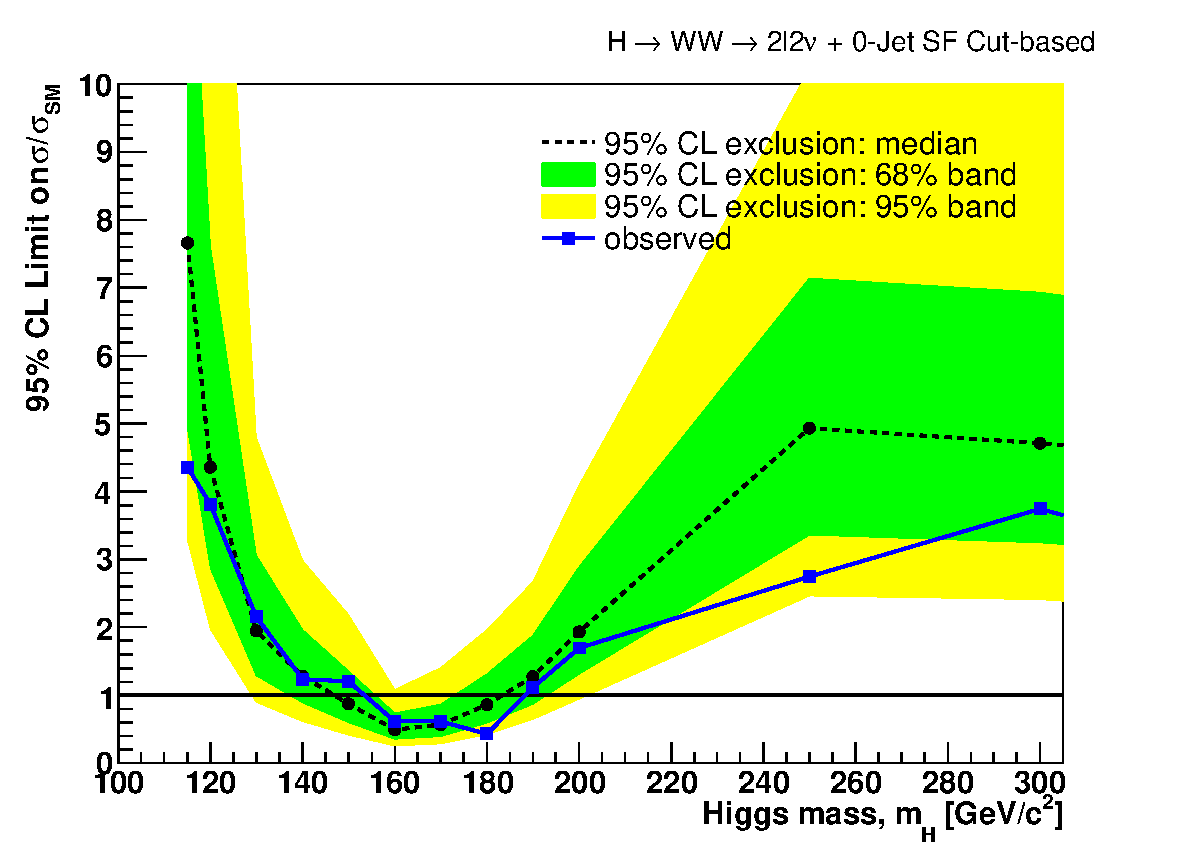
\includegraphics[width=0.48\textwidth]{lp_figures/limits_0j_sf_cut_ana_v6_1500pb_LP_MTCUT80.pdf}}
\subfigure[]{
\centering
\label{subfig:0j_of}
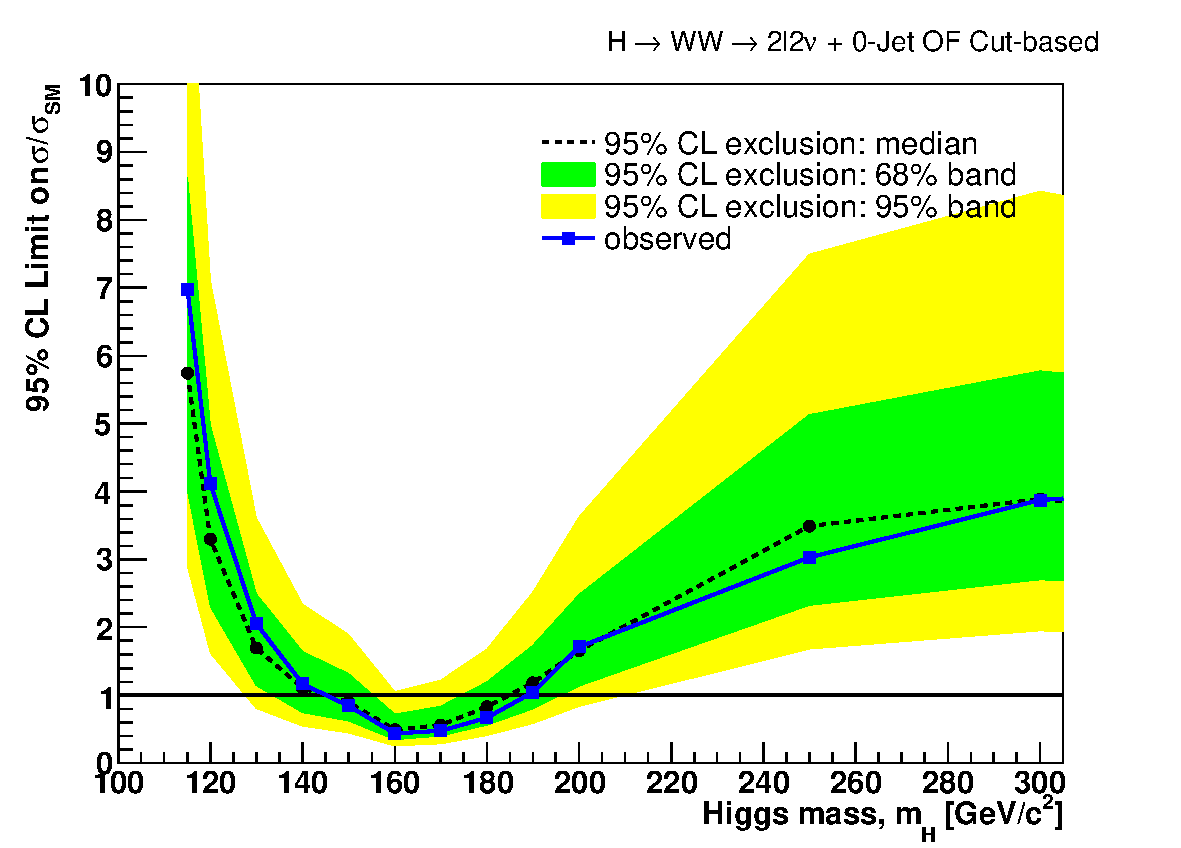
\includegraphics[width=0.48\textwidth]{lp_figures/limits_0j_of_cut_ana_v6_1500pb_LP_MTCUT80.pdf}}
\subfigure[]{
\centering
\label{subfig:1j_sf}
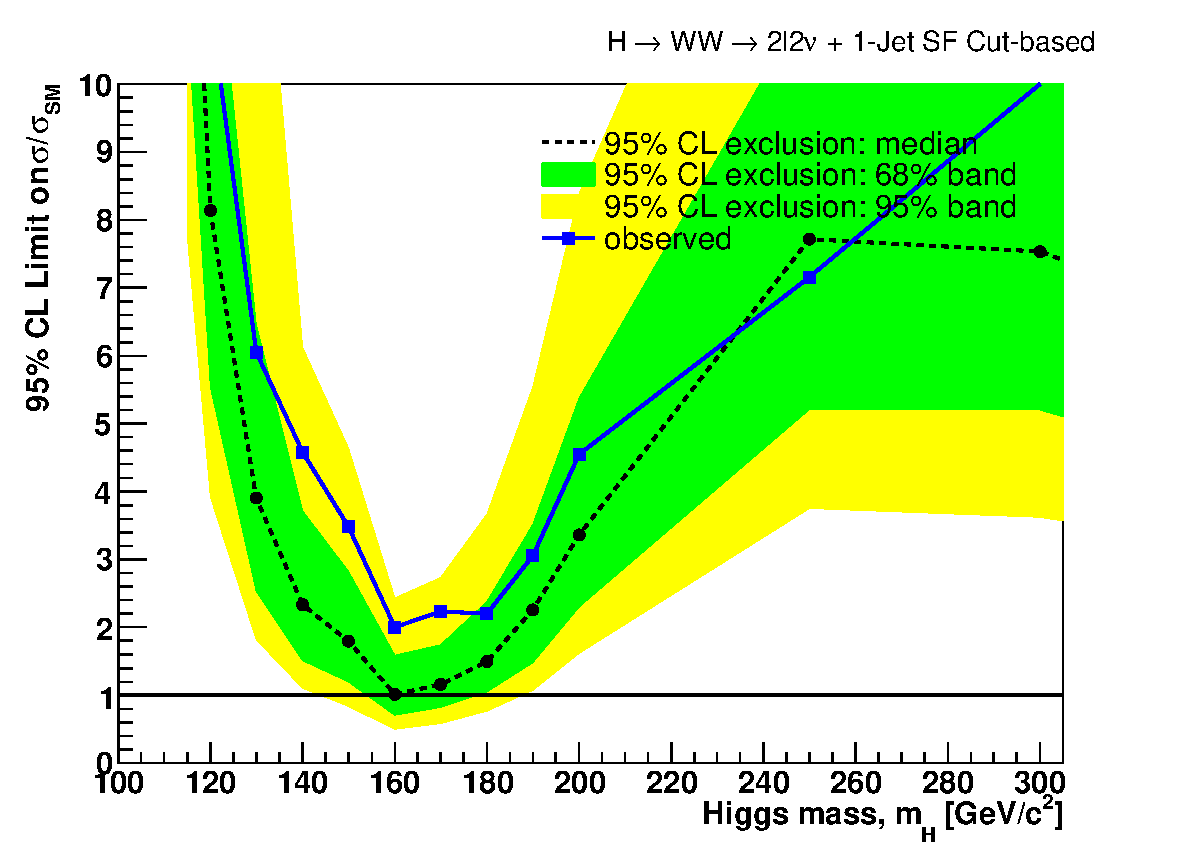
\includegraphics[width=0.48\textwidth]{lp_figures/limits_1j_sf_cut_ana_v6_1500pb_LP_MTCUT80.pdf}}
\subfigure[]{
\centering
\label{subfig:1j_of}
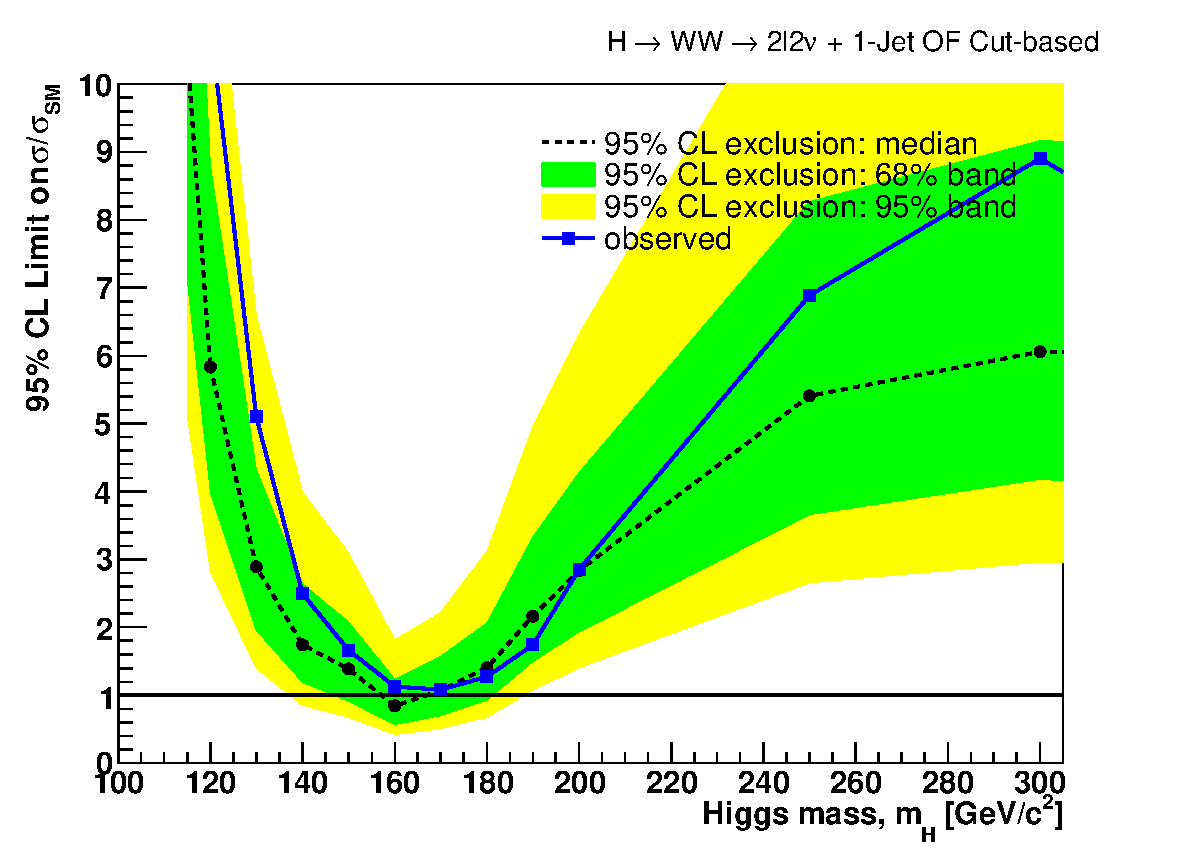
\includegraphics[width=0.48\textwidth]{lp_figures/limits_1j_of_cut_ana_v6_1500pb_LP_MTCUT80.pdf}}
\subfigure[]{
\centering
\label{subfig:2j}
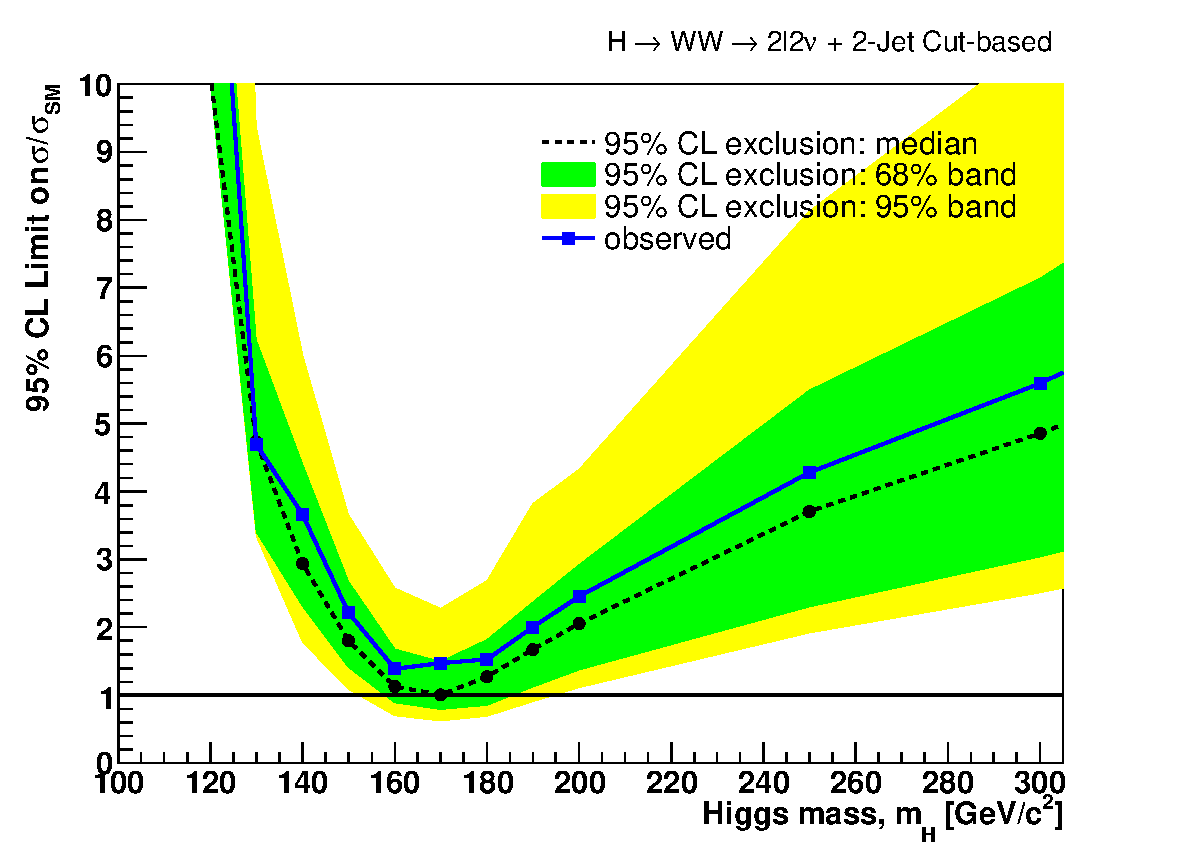
\includegraphics[width=0.48\textwidth]{lp_figures/limits_2j_cut_ana_v6_1500pb_LP_MTCUT80.pdf}}
\subfigure[]{
\centering
\label{subfig:njcomb}
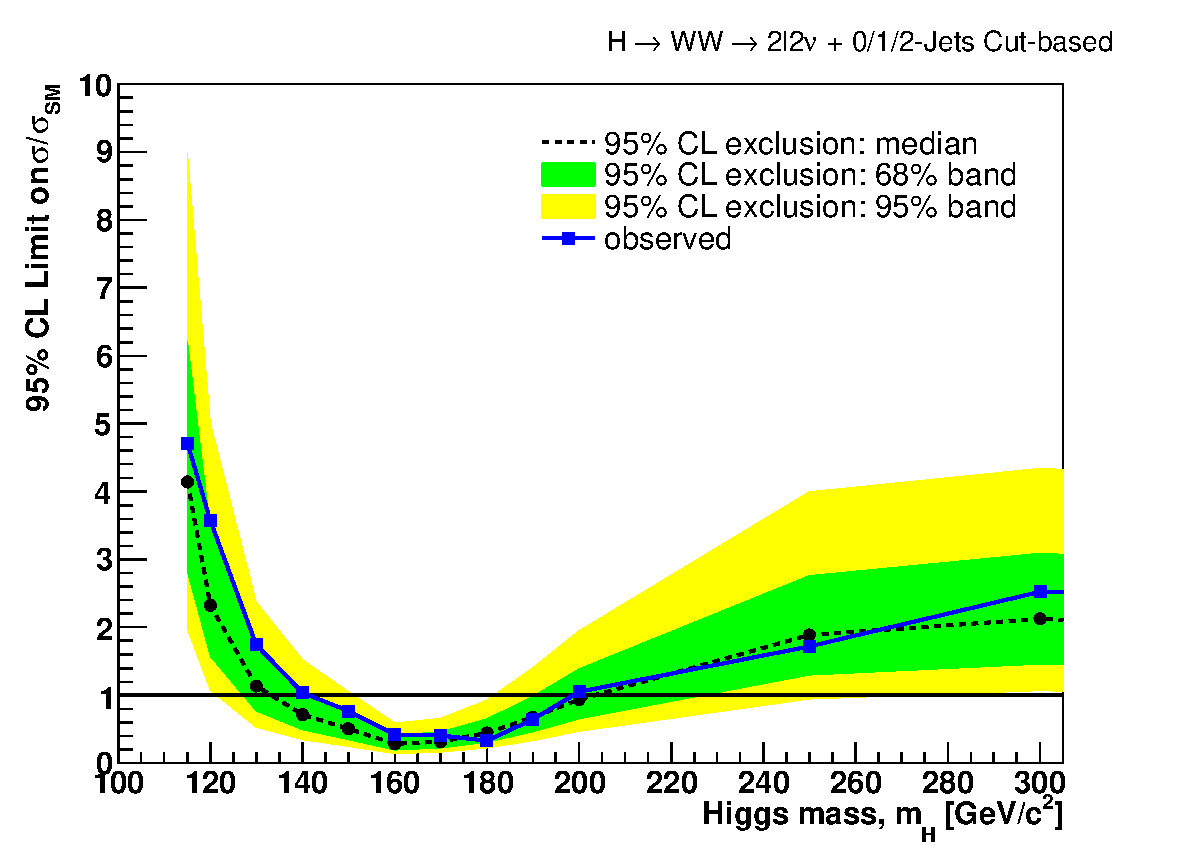
\includegraphics[width=0.48\textwidth]{lp_figures/limits_nj_cut_ana_v6_1500pb_LP_MTCUT80.pdf}}
\caption{Cut-based analysis upper limits at 95\% C.L. using data corresponding to 1.5~$\ifb$.
The limits are shown in 4 final states separately. \subref{subfig:0j_sf}: SF in 0 Jet bin; 
\subref{subfig:0j_of}: OF in 0 Jet bin; \subref{subfig:1j_sf}: SF in 1 Jet bin; 
\subref{subfig:1j_of}: OF in 1 Jet bin; \subref{subfig:2j}: 2 Jet bin; \subref{subfig:nj}: 0/1/2 Jets combined; }
\label{fig:limits_lp_mtcut80_cut}
\end{figure}
%%%%%%%%%%%%%%%%%%%%%%%%%%%%%%
%%%%%%%%%%%%%%%%%%%%%%%%%%%%%%
\begin{figure}[!htbp]
\centering
\subfigure[]{
\centering
\label{subfig:0j_sf}
%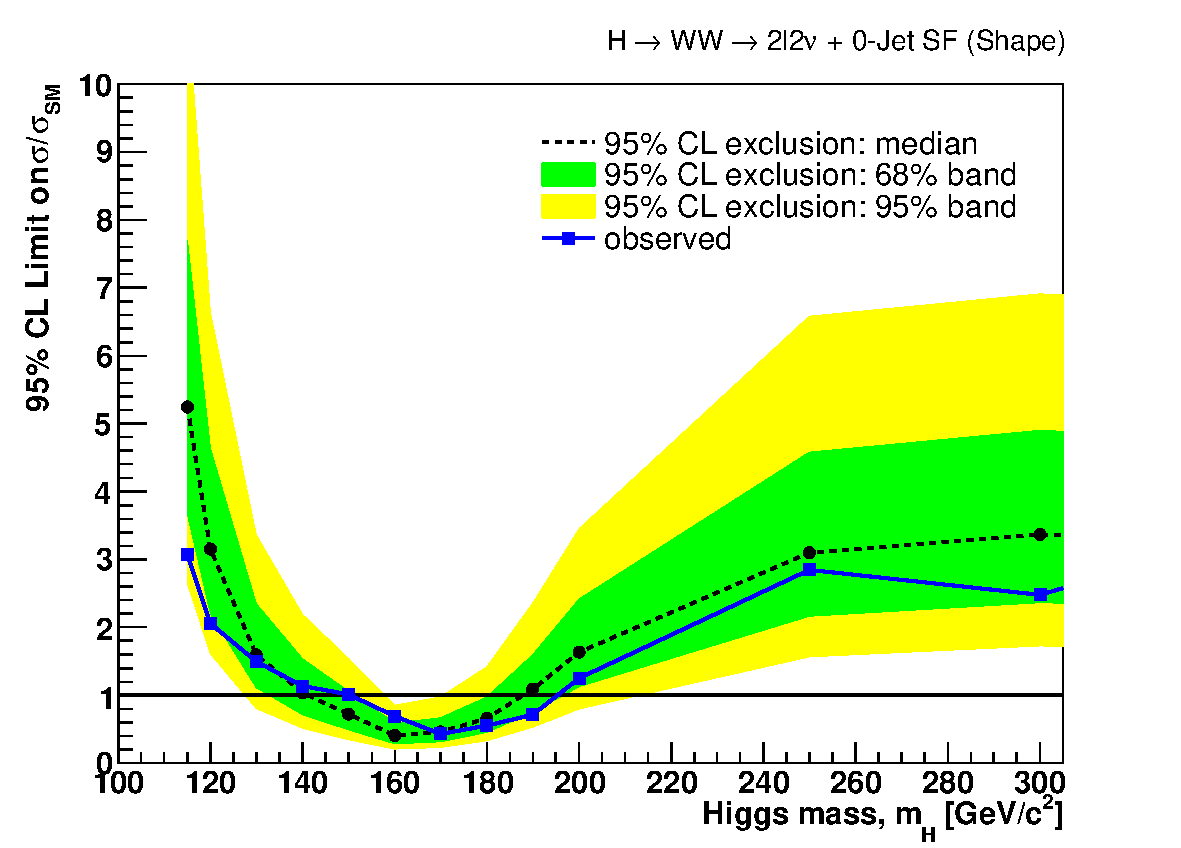
\includegraphics[width=0.48\textwidth]{lp_figures/limits_0j_sf_shape_ana_v6_1500pb_LP_MTCUT80.pdf}
}
\subfigure[]{
\centering
\label{subfig:0j_of}
%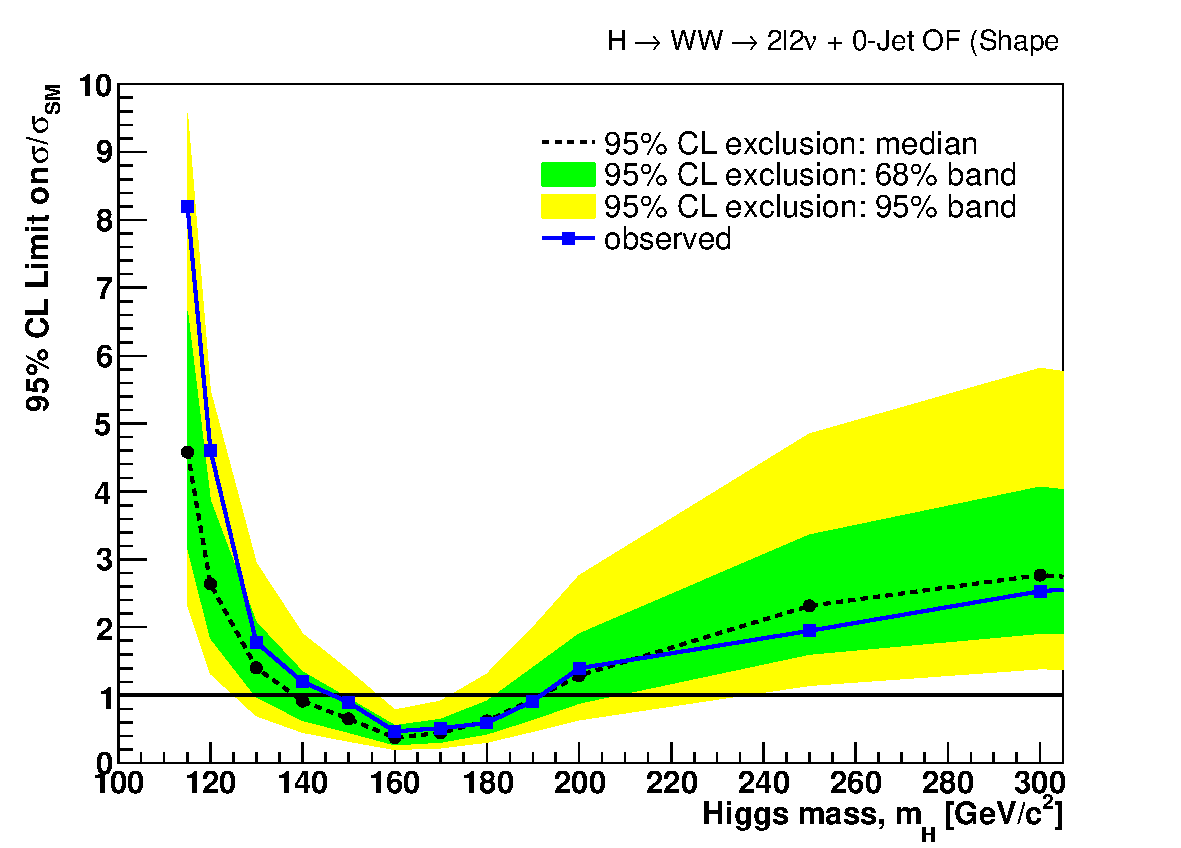
\includegraphics[width=0.48\textwidth]{lp_figures/limits_0j_of_shape_ana_v6_1500pb_LP_MTCUT80.pdf}
}
\subfigure[]{
\centering
\label{subfig:1j_sf}
%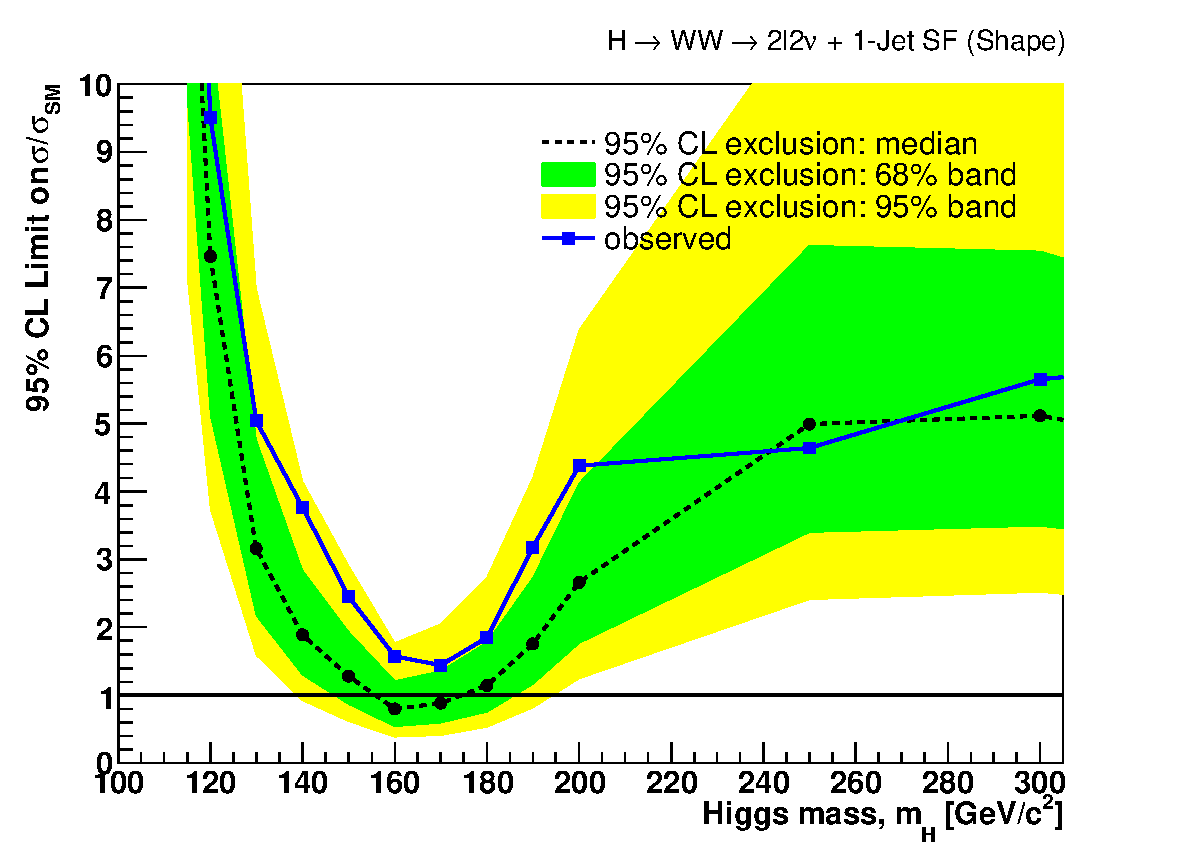
\includegraphics[width=0.48\textwidth]{lp_figures/limits_1j_sf_shape_ana_v6_1500pb_LP_MTCUT80.pdf}
}
\subfigure[]{
\centering
\label{subfig:1j_of}
%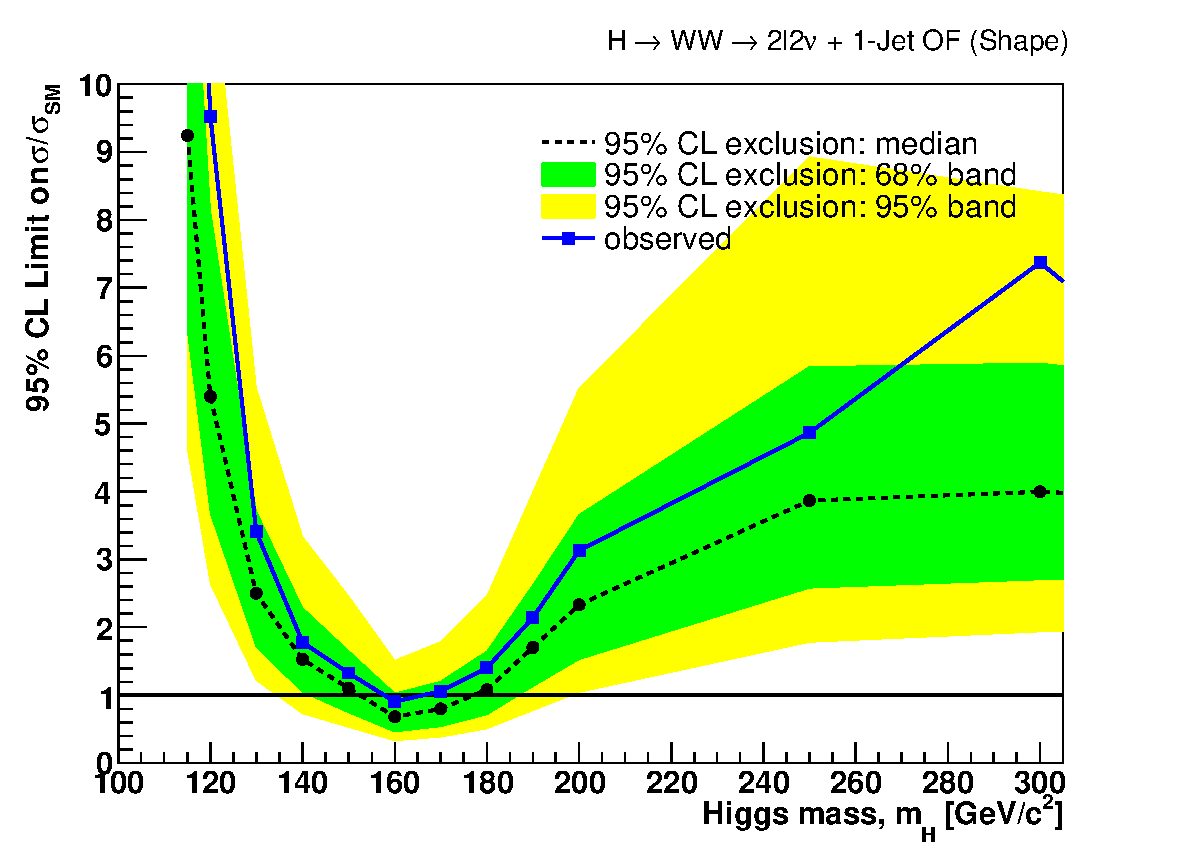
\includegraphics[width=0.48\textwidth]{lp_figures/limits_1j_of_shape_ana_v6_1500pb_LP_MTCUT80.pdf}
}
\subfigure[]{
\centering
\label{subfig:nj}
%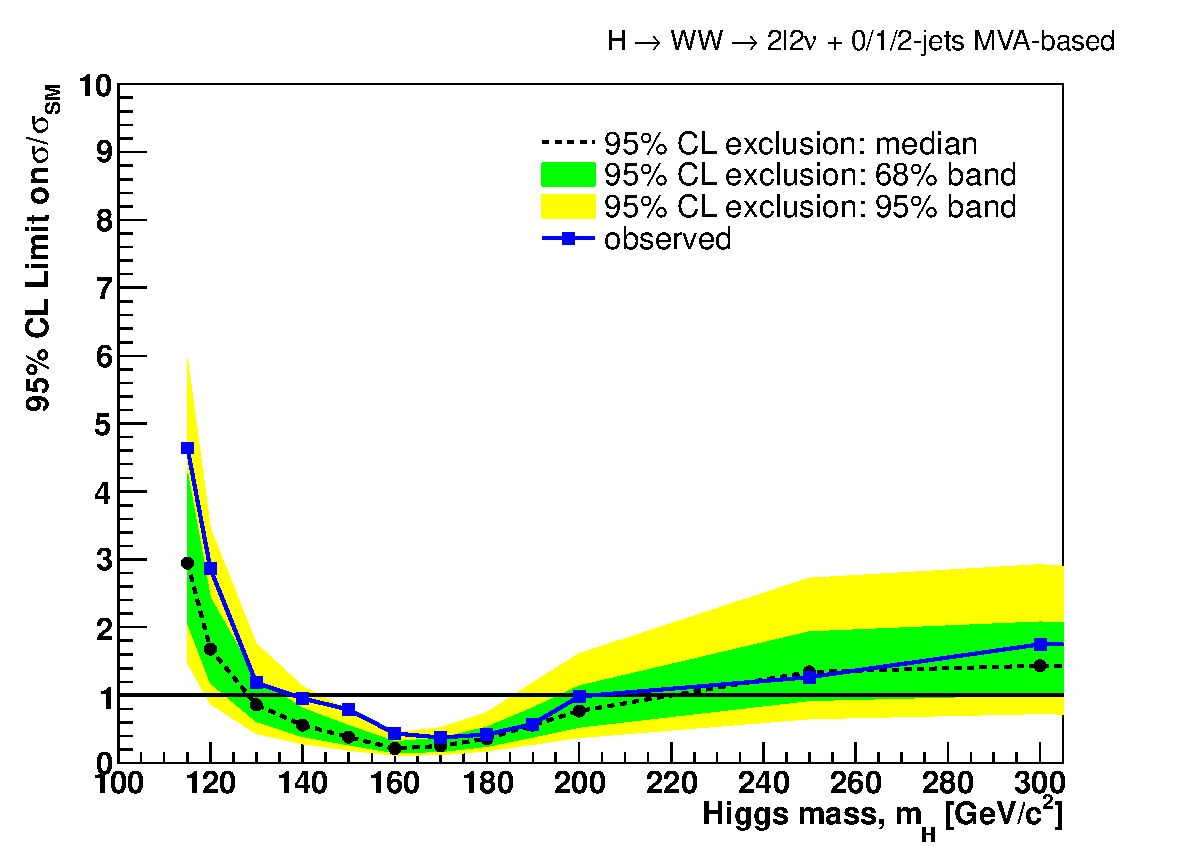
\includegraphics[width=0.48\textwidth]{lp_figures/limits_nj_shape_ana_v6_1500pb_LP_MTCUT80.pdf}
}
\caption{Multivariate based analysis upper limits at 95\% C.L. using data corresponding to 1.5~$\ifb$, 
applying the additional $m_T$ cut.
The limits are shown in 4 final states separately. \subref{subfig:0j_sf}: SF in 0 Jet bin; 
\subref{subfig:0j_of}: OF in 0 Jet bin; \subref{subfig:1j_sf}: SF in 1 Jet bin; 
\subref{subfig:1j_of}: OF in 1 Jet bin; \subref{subfig:nj}: 0/1/2 Jets combined;
}
\label{fig:limits_lp_mtcut80_shape}
\end{figure}
%%%%%%%%%%%%%%%%%%%%%%%%%%%%%%

%%%%%%%%%%%%%%%%%%%%%%%%%%%%%%
\begin{table}
\begin{center}
\begin{tabular}{c c c c c}
\hline\hline
 $m_H$ (GeV) & Observed & Median Expected & 68\% C.L. Band & 95\% C.L. Band \\ \hline
\hline
\multicolumn{5}{c} {0/1/2-Jets Cut-Based}\\
\hline
115 & 4.7 & 4.1 & [2.8, 6.2] & [2.0, 9.0] \\
120 & 3.6 & 2.3 & [1.6, 3.5] & [1.1, 5.0] \\
130 & 1.7 & 1.1 & [0.8, 1.7] & [0.5, 2.4] \\
140 & 1.0 & 0.7 & [0.5, 1.1] & [0.3, 1.5] \\
150 & 0.8 & 0.5 & [0.3, 0.7] & [0.2, 1.1] \\
160 & 0.4 & 0.3 & [0.2, 0.4] & [0.1, 0.6] \\
170 & 0.4 & 0.3 & [0.2, 0.5] & [0.2, 0.7] \\
180 & 0.3 & 0.4 & [0.3, 0.7] & [0.2, 0.9] \\
190 & 0.6 & 0.7 & [0.5, 1.0] & [0.3, 1.4] \\
200 & 1.1 & 0.9 & [0.7, 1.4] & [0.5, 1.9] \\
250 & 1.7 & 1.9 & [1.3, 2.8] & [0.9, 4.0] \\
300 & 2.5 & 2.1 & [1.5, 3.1] & [1.1, 4.3] \\
\hline
\multicolumn{5}{c} {0/1/-Jets Multivariate Based combined with 2-Jet Cut Based}\\
\hline
% FIXME
\hline\hline
\end{tabular}
\end{center}
\caption{Upper limits at 95\% C.L. combining 0, 1 and 2 Jet final states 
for both cut-based and multivariate based analyses, 
shown in Figure~\ref{fig:limits_lp_mtcut80_cut} and Figure~\ref{fig:limits_lp_mtcut80_shape}. 
The results correspond to the 1.5~$\ifb$ data, applying the additional $m_T$ cut. 
} 
\label{tab:limits_lp_mtcut80}
\end{table}
%%%%%%%%%%%%%%%%%%%%%%%%%%%%%%


	
%%%%%%%%%%%%%%%%%%%%%%%%%%%%%%
\begin{table}
\begin{center}
\begin{tabular}{c c c c c}
\hline\hline
 $m_H$ (GeV) & Observed & Median Expected & 68\% C.L. Band & 95\% C.L. Band \\ \hline
\hline
\multicolumn{5}{c} {0-Jet Bin Same Flavor} \\
\hline
115 & 4.4 & 7.7 & [4.9, 13.5] & [3.3, 33.4] \\
120 & 3.8 & 4.4 & [2.9, 7.6] & [2.0, 16.7] \\
130 & 2.2 & 1.9 & [1.3, 3.1] & [0.9, 4.8] \\
140 & 1.2 & 1.3 & [0.9, 2.0] & [0.6, 3.0] \\
150 & 1.2 & 0.9 & [0.6, 1.4] & [0.4, 2.2] \\
160 & 0.6 & 0.5 & [0.3, 0.7] & [0.3, 1.1] \\
170 & 0.6 & 0.6 & [0.4, 0.9] & [0.3, 1.4] \\
180 & 0.4 & 0.9 & [0.6, 1.3] & [0.4, 2.0] \\
190 & 1.1 & 1.3 & [0.9, 1.9] & [0.6, 2.7] \\
200 & 1.7 & 1.9 & [1.3, 2.9] & [0.9, 4.1] \\
250 & 2.8 & 4.9 & [3.4, 7.1] & [2.5, 10.2] \\
300 & 3.7 & 4.7 & [3.2, 6.9] & [2.4, 10.2] \\
\hline
\multicolumn{5}{c} {0-Jet Bin Opposite Flavor} \\
\hline
115 & 7.0 & 5.7 & [4.0, 8.6] & [2.9, 12.6] \\
120 & 4.1 & 3.3 & [2.3, 5.0] & [1.6, 7.1] \\
130 & 2.1 & 1.7 & [1.1, 2.5] & [0.8, 3.6] \\
140 & 1.2 & 1.1 & [0.7, 1.6] & [0.5, 2.3] \\
150 & 0.8 & 0.9 & [0.6, 1.3] & [0.4, 1.9] \\
160 & 0.4 & 0.5 & [0.3, 0.7] & [0.3, 1.0] \\
170 & 0.5 & 0.6 & [0.4, 0.8] & [0.3, 1.2] \\
180 & 0.7 & 0.8 & [0.6, 1.2] & [0.4, 1.7] \\
190 & 1.0 & 1.2 & [0.8, 1.7] & [0.6, 2.5] \\
200 & 1.7 & 1.7 & [1.1, 2.5] & [0.8, 3.6] \\
250 & 3.0 & 3.5 & [2.3, 5.1] & [1.7, 7.5] \\
300 & 3.9 & 3.9 & [2.7, 5.8] & [1.9, 8.4] \\
\hline
\multicolumn{5}{c} {1-Jet Bin Same Flavor} \\
\hline
115 & 18.7 & 15.4 & [11.0, 24.4] & [7.7, 40.3] \\
120 & 11.2 & 8.1 & [5.5, 13.0] & [3.9, 22.8] \\
130 & 6.1 & 3.9 & [2.5, 6.5] & [1.8, 14.2] \\
140 & 4.6 & 2.3 & [1.5, 3.7] & [1.1, 6.1] \\
150 & 3.5 & 1.8 & [1.2, 2.8] & [0.8, 4.6] \\
160 & 2.0 & 1.0 & [0.7, 1.6] & [0.5, 2.4] \\
170 & 2.2 & 1.2 & [0.8, 1.7] & [0.6, 2.7] \\
180 & 2.2 & 1.5 & [1.1, 2.4] & [0.8, 3.7] \\
190 & 3.1 & 2.3 & [1.5, 3.5] & [1.1, 5.5] \\
200 & 4.5 & 3.4 & [2.3, 5.4] & [1.6, 8.4] \\
250 & 7.2 & 7.7 & [5.2, 11.3] & [3.8, 16.1] \\
300 & 10.0 & 7.5 & [5.2, 11.5] & [3.6, 16.8] \\
\hline
\multicolumn{5}{c} {1-Jet Bin Opposite Flavor} \\
\hline
115 & 19.6 & 10.5 & [7.1, 15.4] & [5.1, 22.5] \\
120 & 10.9 & 5.8 & [4.0, 8.8] & [2.8, 12.8] \\
130 & 5.1 & 2.9 & [2.0, 4.3] & [1.4, 6.6] \\
140 & 2.5 & 1.7 & [1.2, 2.6] & [0.8, 4.0] \\
150 & 1.7 & 1.4 & [0.9, 2.1] & [0.7, 3.1] \\
160 & 1.1 & 0.8 & [0.6, 1.2] & [0.4, 1.8] \\
170 & 1.1 & 1.1 & [0.7, 1.6] & [0.5, 2.2] \\
180 & 1.3 & 1.4 & [0.9, 2.1] & [0.7, 3.1] \\
190 & 1.7 & 2.2 & [1.5, 3.3] & [1.1, 5.0] \\
200 & 2.9 & 2.8 & [1.9, 4.3] & [1.4, 6.3] \\
250 & 6.9 & 5.4 & [3.7, 8.3] & [2.7, 12.1] \\
300 & 8.9 & 6.1 & [4.2, 9.2] & [3.0, 13.8] \\
\hline\hline
\end{tabular}
\end{center}
\caption{Cut based upper limits at 95\% C.L. in 0 and 1 Jet final state, 
using data corresponding to 1.5~$\ifb$ shown in 
Figure~\ref{fig:limits_lp_mtcut80_cut}. We apply the additonal $m_T$ cut.}  
\label{tab:limits_lp_mtcut80_cut_splitflavor}
\end{table}
%%%%%%%%%%%%%%%%%%%%%%%%%%%%%%

%%%%%%%%%%%%%%%%%%%%%%%%%%%%%%
\begin{table}
\begin{center}
\begin{tabular}{c c c c c}
\hline\hline
 $m_H$ (GeV) & Observed & Median Expected & 68\% C.L. Band & 95\% C.L. Band \\ \hline
\hline
\multicolumn{5}{c} {0-Jet Bin Same Flavor} \\
\hline
% FIXME
\hline
\multicolumn{5}{c} {0-Jet Bin Opposite Flavor} \\
\hline
% FIXME
\hline
\multicolumn{5}{c} {1-Jet Bin Same Flavor} \\
\hline
% FIXME
\hline
\multicolumn{5}{c} {1-Jet Bin Opposite Flavor} \\
\hline
% FIXME
\hline\hline
\end{tabular}
\end{center}
\caption{Multivariate based upper limits at 95\% C.L. in 0 and 1 Jet final state, 
using data corresponding to 1.5~$\ifb$ shown in 
Figure~\ref{fig:limits_lp_mtcut80_shape}. We apply the additional $m_T$ cut.} 
\label{tab:limits_lp_mtcut80_shape_splitflavor}
\end{table}
%%%%%%%%%%%%%%%%%%%%%%%%%%%%%%
